\section{需求和功能点}
课题系统主要的服务对象是使用这个项目的老师和学生,下面针对课题系统目前
的受众和课题系统的目标,提出详细的需求说明。

\subsection{功能性需求}
\subsubsection{词法分析的动画设计}
\begin{itemize}
\item 明辨词法单元、模式以及词素的动画,能够将词法单元、模式以及词素
  从动画上面说明清楚,能够实现适当的提示,包括鼠标移动上去的提示,
  本身的字幕提示以及任何其他合理的提示。
  \begin{table}[!hbp]
  	\centering
  	\begin{tabular}{c|c|c}
  		\hline
  		词法单元 & 非正式描述 & 词素示例\\
  		\hline
  		if & 字符i、f & if\\
  		\hline
  		id & 字母开头的字母或数字串 & isPrepare\\
  		\hline
  		literal & 在俩个双引号之间的除双引号外的任意字符 & ``I'm done"\\
		\hline
  	\end{tabular}
  	\caption{词法单元的例子}
  \end{table}
  \begin{figure}[!htb]
  	\centering
  	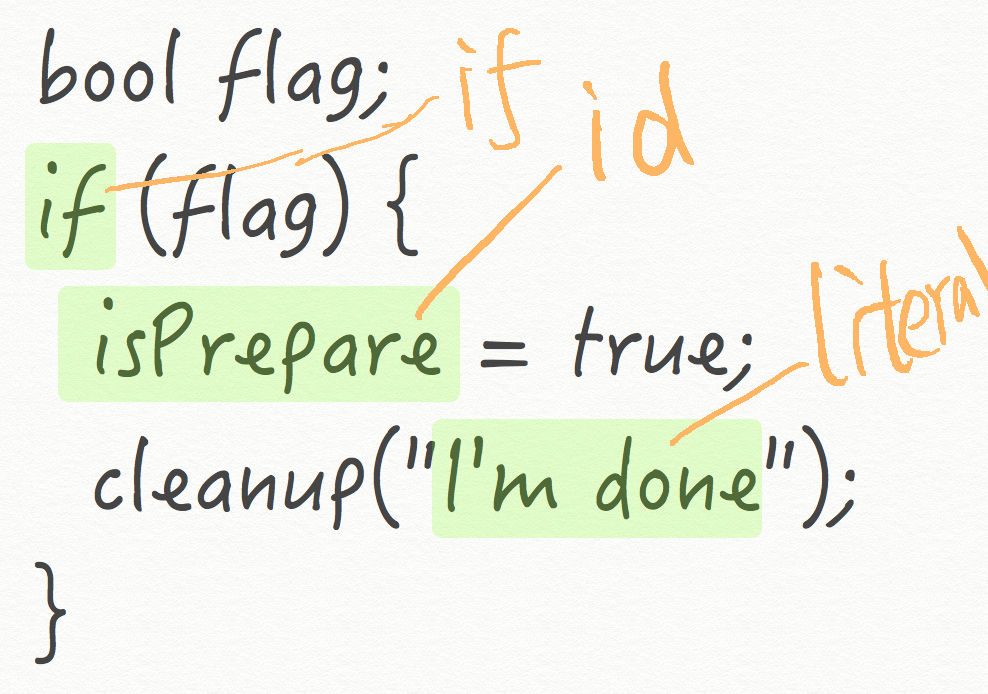
\includegraphics[width=0.7\linewidth]{img/lexical.png}
  	\caption{当鼠标放上去的时候,应该显示橘黄色的内容}
  	\label{fig:lexical.png}
  \end{figure}
\item 输入缓冲动画设计,说明清楚缓冲的作用,在动画中要能够清晰标明指针
  的位置,缓冲区的特点,能够让用户自定义输入文本的内容,也能够提供从不
  同的地方输入文本的内容的功能,详细的要求参见对文法输入的要求。可以提
  供一定的算法步骤,进行算法演示,这部分可选,因为输入缓冲的目的是让同
  学理解输入缓冲,而输入缓冲的算法实践本身比较简单。
    \begin{figure}[!htb]
    	\centering
    	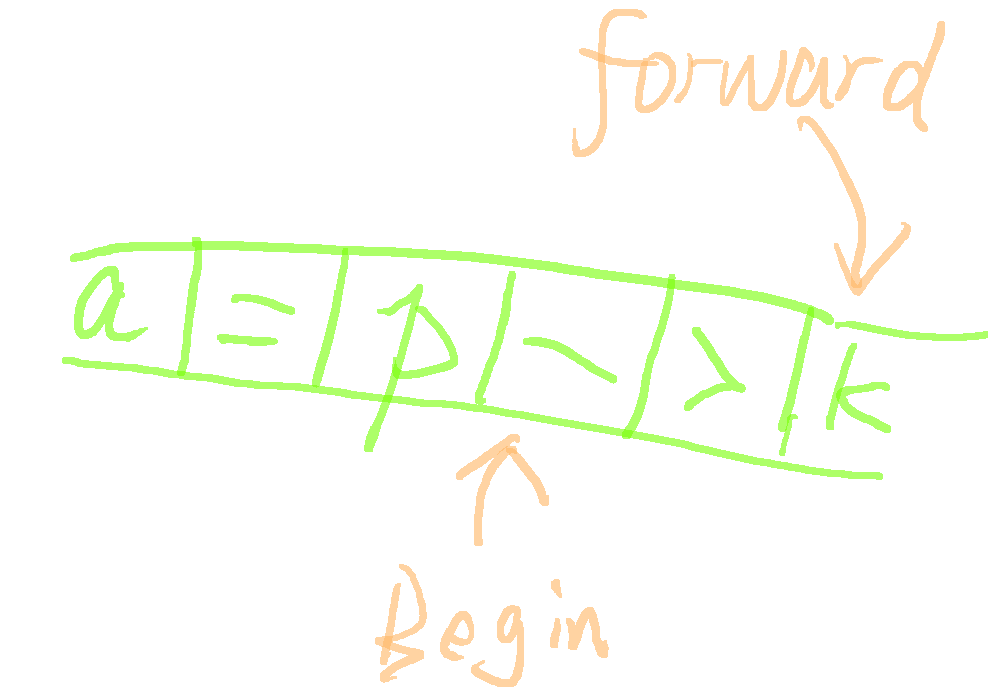
\includegraphics[width=0.7\linewidth]{img/buffer.png}
    	\caption{动画应当演示begin和forward指针的移动}
    	\label{fig:buffer.png}
    \end{figure}
\item 词法单元的归约的动画设计,使用动画来说明词法单元归约的各种名词,
  即通过一个动画,展示串的各个部分分别指的是哪些内容,通过动画,来说明
  语言上的运算是怎么样子的。这里可以适当加上对正则匹配过程的动画演示,
  可以参考已有的开源项目,不一定做成动画,可以做成匹配过程可以看到的匹
  配元素,就已经能够比较清晰说明正则匹配的内容。
      \begin{figure}[!htb]
      	\centering
      	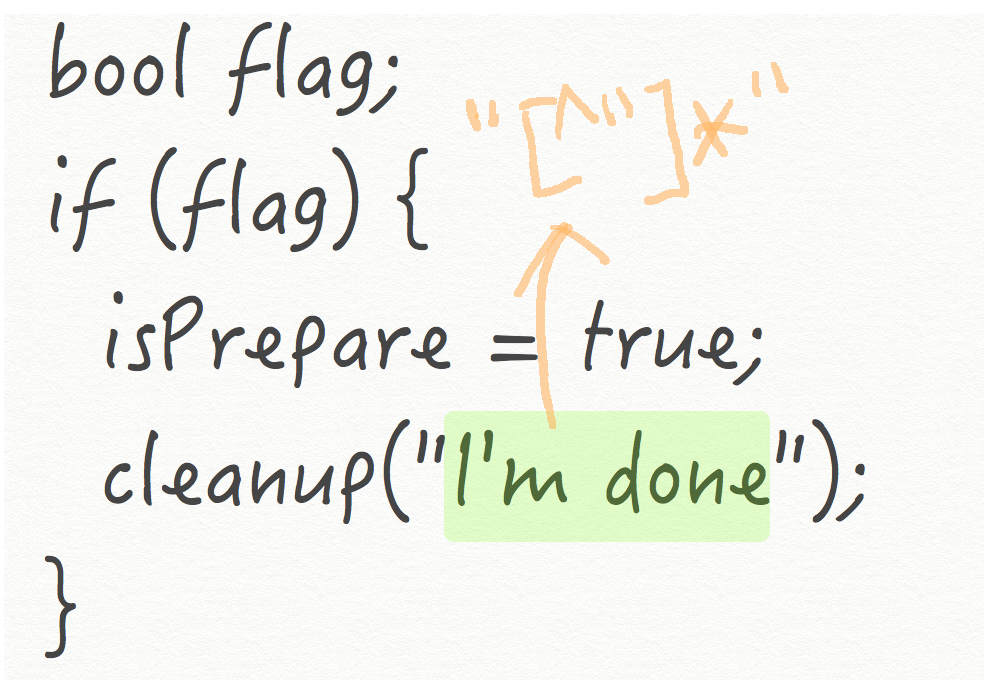
\includegraphics[width=0.7\linewidth]{img/reduction.png}
      	\caption{用高亮标出匹配的词法单元,在鼠标悬浮在上面的时候显示正则表达式}
      	\label{fig:reduction.png}
      \end{figure}
\item 词法单元的识别的动画设计,用一个动画,配合词素、词法单元名字、属
  性值的内容,来演示词法单元配合的时候应该如何去识别每一个词法单元,他
  们是怎么被标记出来的可以做出成动画,辅助一些流水线的效果。另外还需介
  绍基于状态转换图的词法分析的体系结构,这部分可以用动态的状态图来展示
  出来它的工作效果,可以辅以代码来查看当前执行的情况。
        \begin{figure}[!htb]
        	\centering
        	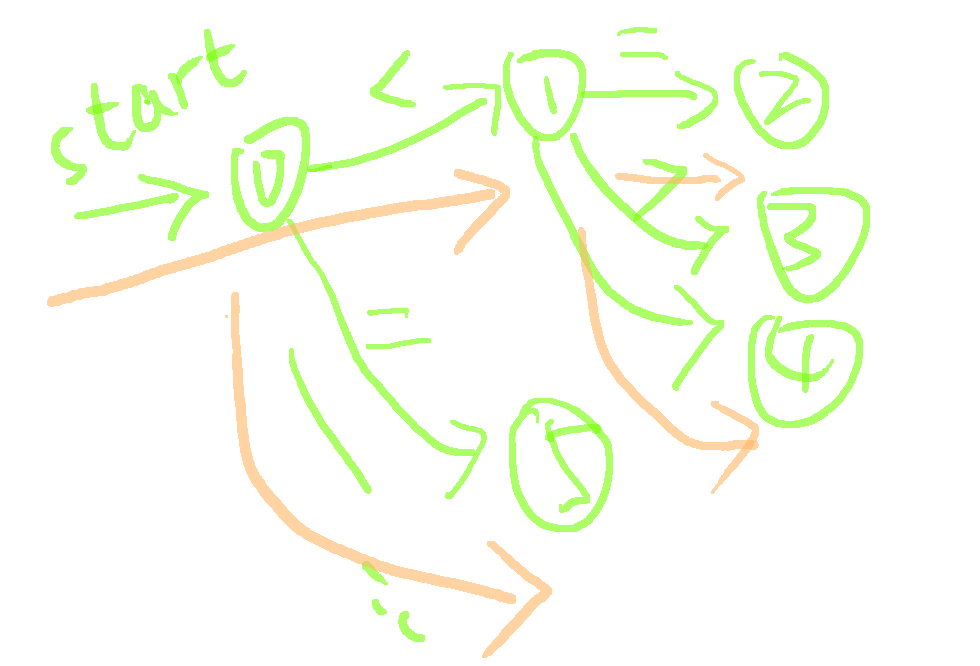
\includegraphics[width=0.7\linewidth]{img/recognize.png}
        	\caption{由人工输入(教师)状态图,演示特定词法单元如何匹配}
        	\label{fig:recognize.png}
        \end{figure}
\item 有穷自动机的动画设计,这部分内容基础要求是通过算法步骤一步步展示
  如何进行子集构造,在这个基础上,应该能完成更高的目标,利用算法步骤得
  到的结果,来动态构造一个动态图。最后应该要点名字符串的算法效率,可以
  做一个在线的测试给出一个测试结果,让同学们能直观的理解字符串处理的效
  率。
\end{itemize}
\subsubsection{语法分析的动画设计}
\begin{itemize}
\item 语法分析树的动画设计,这部分不具体讲解算法,因此就展示任意给定的
  一段代码,再给定一个文法,展示下一个语法分析树的展开,预先应该存有多
  个代码段以及匹配的文法。而且,能够在一定范围内处理异常的情况,指的不
  是能修正错误,而是如果发生文法和代码不匹配的情况,能够告之用户这俩者
  之间有不匹配的情况,可以根据后面的算法,指明在匹配到哪里的时候出现错
  误。
          \begin{figure}[!htb]
          	\centering
          	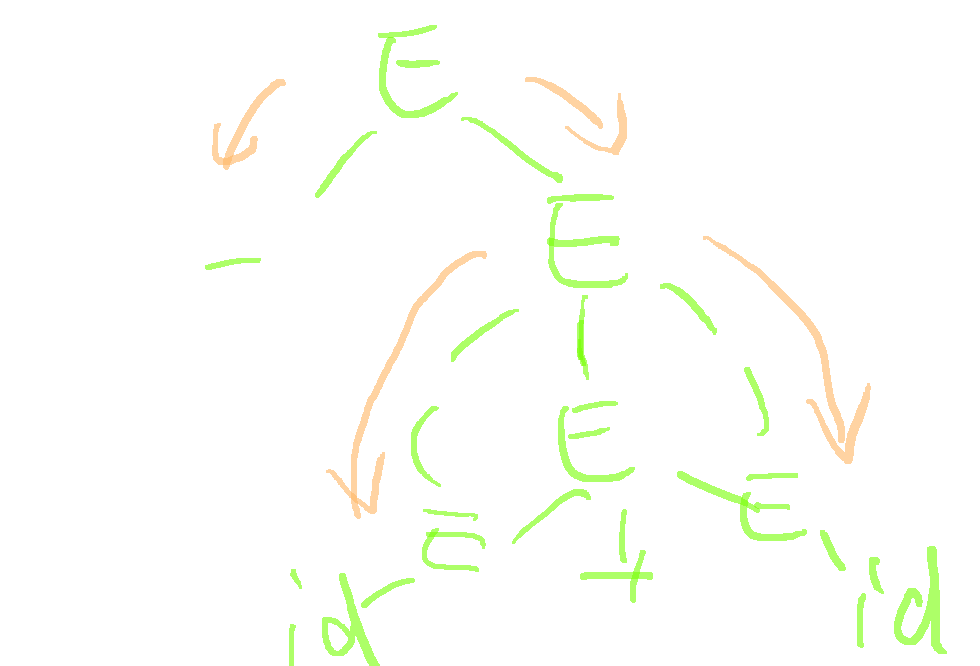
\includegraphics[width=0.7\linewidth]{img/analyze.png}
          	\caption{对给定文法、代码生成语法分析树,展示树展开的动画}
          	\label{fig:analyze.png}
          \end{figure}
\item 左递归消除的动画设计,这部分动画应该直接包括直接左递归和间接左递
  归的情况。能够用动画展示出来算法的每一步骤针对的是哪些元素,并且可以
  指示算法当前进行到的位置,以及可以停止获取当前的各项变量的情况。
            \begin{figure}[!htb]
            	\centering
            	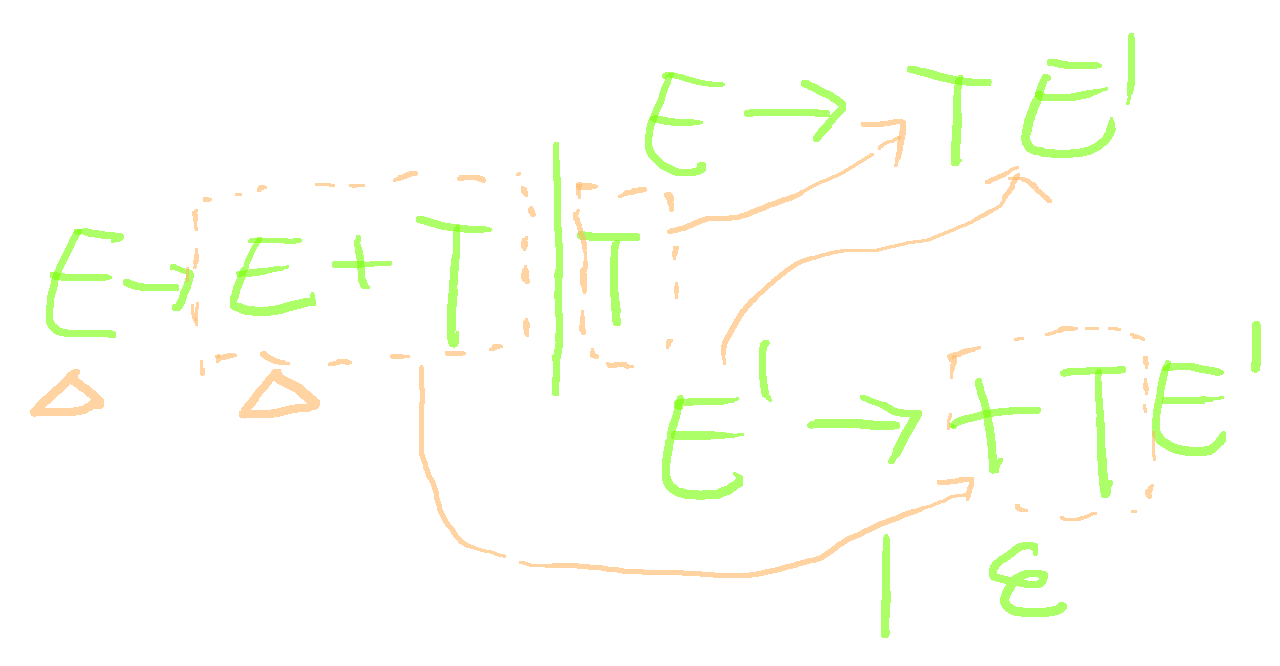
\includegraphics[width=0.7\linewidth]{img/leftrecursive.png}
            	\caption{动画中应表达出左递归消除进行的过程}
            	\label{fig:leftrecursive.png}
            \end{figure}
\item 提取左公因子的动画设计,这个算法内容比较简单,动画可以按照算法的
  进程,演示每一个公因子被找到的过程以及被提取的过程。
\item FIRST和FOLLOW集合构造的动画设计,根据构造FIRST集和FOLLOW集的算法,
  依次计算每一个非终结符号的集合,可以以多个集合图的方式来演示动画,表
  现出如何找到这些集合的过程。
              \begin{figure}[!htb]
              	\centering
              	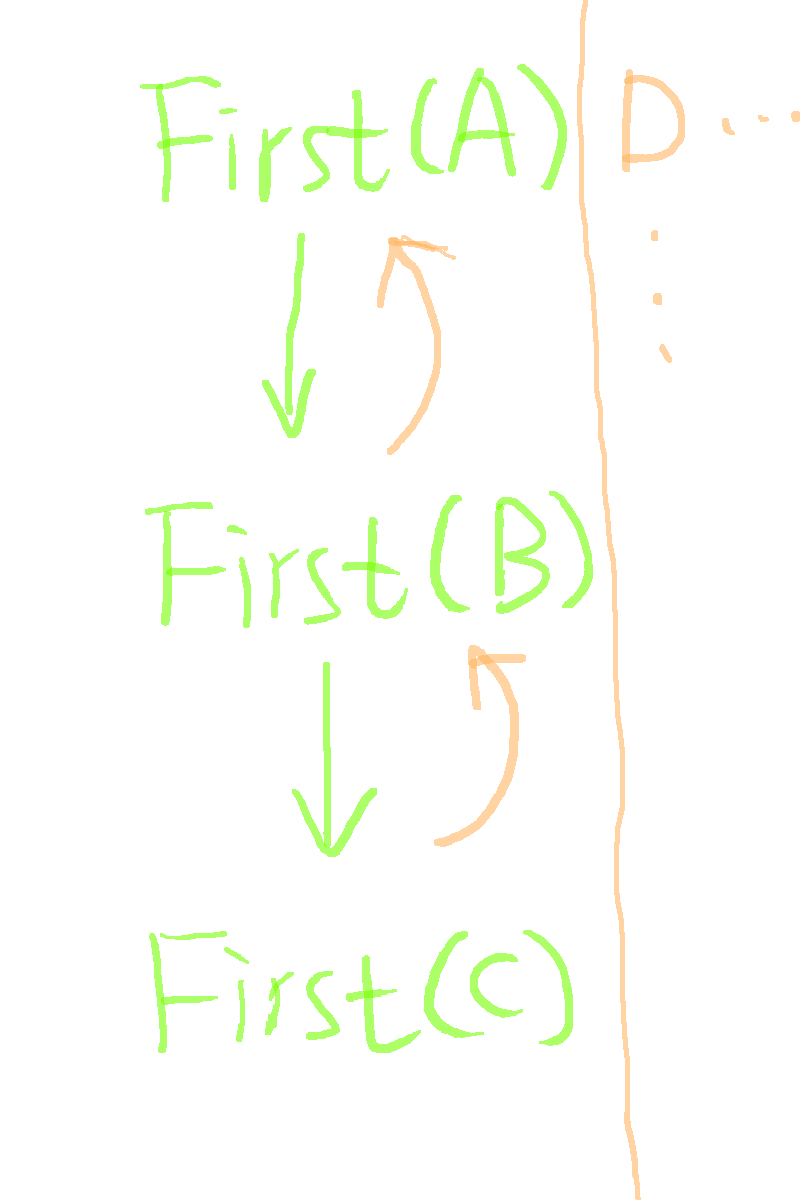
\includegraphics[width=0.4\linewidth]{img/first.png}
              	\caption{将求first的回溯过程表现出来}
              	\label{fig:first.png}
              \end{figure}
\item 各类文法的动画设计,对于使用的每一个文法,我们可以设计出一个简短的动
  画来说明它的内涵。另一个要求是做出它的预测分析表,用FIRST和FOLLOW集
  合来逐步构建一个,在动画中展示出,如何构建每一行每一列的元素,动画应
  与输入符号相关联的算法执行情况。可以设计出栈的动画,方便用户可以查看
  到进出栈的情况。
\end{itemize}
\subsubsection{用户输入内容管理}
支持用户将输入内容暂存在系统中,方便用户进行演示,或者自己观看。输入内
容存储这块有一些具体的要求,下面以文法存储作为例子进行解释。其他的暂存
内容,也应该满足输入、验证、获取这三方面的要求。
\begin{itemize}
\item 支持从多种渠道输入文法,分别应该有直接输入文法,从文件中获取文法,
  从URL中获取文法,其中文件中获取文法应该支持直接拖拽来上传文法以及从
  文件管理器中选择文法这俩种方式。
\item 支持文法的保存与记录,可以对文法进行命名和归类,可以分享文法给其
  他人,可以对文法进行评注以及说明。
\item 支持对文法进行报错提示,指的是文法不符合既定的格式,具体的格式要
  求在程序内说明。
\item 
\end{itemize}
\subsection{非功能性需求}
\subsubsection{健壮性}
系统应该具有一定的稳定性,在这个系统中,主要指的是,不会因为用户无意间
的某些操作而导致动画出现问题,界面出现卡顿的现象。在系统崩溃后,会尽可
能保留用户当前使用的数据,提供给用户一个稳定可靠的环境。
\subsubsection{可用性}
系统应该是高度可用的,具体指的是,用户应该可以在任何现代浏览器上都可以
打开我们课题项目中的web系统。用户可以很方便使用系统中提供的每一个功能,
而不会产生明显的使用障碍。系统应该改善用户可能比较困惑的地方的设计,在
无法做到明确的系统使用时,应该使用适当的辅助机制,比如提供帮助文档,等
方式来教会用户如何使用这个系统。
\subsubsection{可重用性}
系统应该具有高度可重用性,主要分成以下俩个方面。一个方面是,在系统内部,
动画应该具有可重用性,一个动画的的制作,可以给多个地方提供重用,又能提供
适当针对实际情况的改变。另一方面是,系统应该能够被外部程序重用,比如现
有的MOOC系统应该要能很容易将系统的内容重用,而不需要大量改写现有的组件。
\subsubsection{可维护性}
系统应该容易维护,应用充分利用面向对象和软件工程中的开发方法,使得系统
易于原来的开发者以及新的维护者维护。系统应该为此提供相应的开发文档,使
用模块化的建设,减少模块之间的耦合,增强模块的内容,增强模块的可扩展性,
提供方便的动画开发流程等等。
\subsubsection{可扩充性}
系统应该具有高度的可扩充性,可以从两个方面着手,一方面是开发者应该能提
供新的模块,使得系统能有更多的功能,而用户应该能够通过自己编写一些小的
脚本,实现系统一些辅助的功能。